% =====================================================================
%  HotMobile 2027 — COMBINED position paper (CPU + Apple Silicon).
%  Drafted 2026-08-06. Separate from main.tex (the Paper-1-only port).
%  Deadline: 9 Oct 2026 11:59pm AoE · <=6pp · sigconf 10pt · non-anonymous
%  Build:  tectonic combined.tex     (or: latexmk -pdf combined.tex)
%  TODO before submission:
%    (1) Figure 1 — combined prefill-fraction curve for both platforms,
%        generated from the two released datasets. Placeholder below.
%    (2) Swap in HotMobile's official 10pt-amended acmart template if provided.
%    (3) Add CCS concepts (required for camera-ready, optional at submission).
% =====================================================================
\documentclass[sigconf,nonacm,10pt]{acmart}

\usepackage{booktabs}
\usepackage{graphicx}
% acmart already provides amsmath, amssymb, hyperref, natbib, xcolor

\settopmatter{printacmref=false}
\renewcommand\footnotetextcopyrightpermission[1]{}
\pagestyle{plain}
\setcopyright{none}
\emergencystretch=2em

\begin{document}

\title{Your Latency Intuition Doesn't Port: Prefill/Decode Inversion
Between CPU and Apple Silicon}

\author{Bapista Khan}
\affiliation{%
  \institution{Collab-Foundry}
  \country{}}
\email{bapistakhan@gmail.com}
\renewcommand{\shortauthors}{Bapista Khan}

\begin{abstract}
On-device language models are increasingly deployed for privacy, offline operation and cost, yet the latency
intuition the community carries is inherited from datacentre GPU serving, where autoregressive \emph{decode}
dominates. We instrumented end-to-end inference on two on-device platforms and found that neither matches that
intuition---and, more usefully, that they do not match \emph{each other}. On a CPU-only machine, prompt
\emph{prefill} grows from 38\% of end-to-end latency at 55 tokens to \textbf{95\%} at 2{,}336 tokens: latency is
governed by how much the model \emph{reads}. On an 8\,GB Apple Silicon device the balance inverts---at short and medium
context the system is \textbf{decode-bound} (prefill only 14--20\% of latency), per-token prefill is up to
\textbf{12$\times$ cheaper} than decode, and beyond
$\sim$2{,}029 tokens decode throughput \emph{collapses} from 49 to 13\,tok/s as weights plus KV cache exhaust
unified memory. The two platforms are not two points on one curve; they are two regimes, with different binding
constraints---compute on one, memory on the other. We argue that this has immediate consequences for how the
mobile systems community benchmarks, schedules and budgets on-device inference, and that single-number
throughput reporting actively conceals the effect. Harnesses and raw data for both platforms are released.
\end{abstract}

\keywords{on-device inference, mobile systems, LLM, latency, prefill, memory wall, measurement}

\maketitle

% =====================================================================
\section{Introduction}
% =====================================================================

Running language models on the device rather than in the datacentre is no longer exotic. Privacy requirements,
offline operation, and the cost of inference at scale have all pushed capable models onto phones, laptops and
edge hardware~\cite{xu2024ondevicereview,liu2024mobilellm,xue2024powerinfer2}. The engineering intuition that
travelled with them, however, did not come from those devices. It came from GPU serving, where the dominant
cost is autoregressive \emph{decode}, and where the field's optimisation effort---batching, paged attention,
speculative decoding---has been directed accordingly~\cite{kwon2023pagedattention,leviathan2023speculative}.

We took that intuition to two on-device platforms and measured it. It failed on both, in opposite directions.

On a CPU-only machine with no GPU, \emph{prefill}---the single parallel pass that reads the prompt---grows from
38\% of end-to-end latency on a 55-token prompt to \textbf{95\%} at 2{,}336 tokens, crossing 90\% beyond roughly
1{,}300 tokens. Decode throughput stays essentially flat at 11--12\,tok/s throughout. End-to-end latency is
therefore governed by \emph{context length}, not output length: the inverse of the GPU-era assumption.

On an 8\,GB Apple Silicon device the picture inverts again. At short and medium context the system is
\emph{decode-bound}: prefill accounts for only \textbf{14--20\%} of latency. Prefill overtakes decode only deep
into long context and caps at \textbf{73--80\%}, never reaching CPU levels. Per token, reading is up to
\textbf{12$\times$ cheaper} than writing. And past roughly 2{,}029 tokens, decode throughput does not degrade
gracefully---it \emph{collapses}, from 49\,tok/s to 13\,tok/s, as model weights plus a growing KV cache exceed
available unified memory.

The point of this paper is not that either measurement is surprising in isolation. It is that \textbf{there is
no portable answer}. A practitioner who learns where the time goes on one on-device platform learns something
that is actively misleading about the next one. The binding constraint is compute on one and memory on the
other, and no single number---least of all ``tokens per second''---distinguishes them.

\paragraph{Contributions.}
\begin{itemize}
  \item We characterise prefill/decode balance end-to-end on two on-device platforms and show the bottleneck
        \emph{inverts} between them (\S\ref{sec:two}).
  \item We give the mechanism that explains the inversion, and argue the two platforms represent distinct
        regimes rather than positions on a continuum (\S\ref{sec:why}).
  \item We draw out what follows for mobile systems practice---benchmarking, placement, context budgeting, and
        treating the memory wall as a discontinuity rather than a tuning parameter (\S\ref{sec:implications}).
  \item We release both harnesses and all raw data (\S\ref{sec:repro}).
\end{itemize}

% =====================================================================
\section{Two Platforms, Two Answers}
\label{sec:two}
% =====================================================================

\paragraph{Setup.} Both studies sweep prompt length from 55 to 2{,}336 tokens with five repetitions per point,
discarding warm-up runs, and instrument prefill and decode separately end to end. Platform~A is a CPU-only
machine (AMD Ryzen~7 8845HS, 8 cores / 16 threads, 14\,GiB) running quantized builds through
\texttt{llama.cpp}~\cite{gerganov2023llamacpp}. Platform~A measures Qwen2.5-7B, Llama-3.1-8B and Gemma2-9B.
Platform~B is an 8\,GB MacBook Air running 4-bit MLX builds of Qwen2.5-Instruct at 0.5B, 1.5B and 3B---a
deliberate size sweep on a device where the larger families do not comfortably fit, which is itself part of the
finding. Every published number traces to a released raw-results file.

\begin{table}[t]
\caption{The same measurement, two platforms. The binding constraint changes, and with it what a developer
should optimise.}
\label{tab:contrast}
\small
\begin{tabular}{@{}lll@{}}
\toprule
 & \textbf{A: CPU (14\,GiB)} & \textbf{B: Apple Silicon (8\,GB)} \\
\midrule
Prefill share      & 38\% $\rightarrow$ \textbf{95\%} & \textbf{14--20\%} $\rightarrow$ 73--80\% \\
Decode throughput  & flat $\sim$11--12\,tok/s          & 49 $\rightarrow$ \textbf{13}\,tok/s \\
Per-token balance  & prefill expensive                 & prefill $\sim$\textbf{12$\times$} cheaper \\
Crossover (50\%)   & below 55\,tok                     & \textbf{1{,}029}\,tok (0.5B) $\rightarrow$ \textbf{329} (3B) \\
Governed by        & context length                    & context \emph{and} memory headroom \\
Binding constraint & \textbf{compute}                  & \textbf{memory} \\
\bottomrule
\end{tabular}
\end{table}

Table~\ref{tab:contrast} is the paper. Read down either column and a coherent optimisation strategy follows;
read across and the two strategies contradict each other.

\paragraph{Model size moves the crossover, but not the regime.} On Platform~A, Llama-3.1-8B and Gemma2-9B sit at
95--96\% prefill at $\sim$1{,}300 tokens, matching Qwen2.5-7B. On Platform~B the crossover shifts with size---moving
\emph{earlier} for larger models: $\sim$1{,}029 tokens at 0.5B against $\sim$329 at 3B. The regime does not
change---all three are decode-bound at typical context lengths---but the point at which prefill starts to matter
arrives sooner the bigger the model gets.

\paragraph{It is not vendor-specific either.} We repeated the CPU sweep on a second vendor (Intel Comet Lake).
Prefill dominance reproduces, and is if anything stronger.

\paragraph{Quantization does not behave the way the folklore says.} On Platform~A, prefill \emph{speed} is
non-monotonic in footprint: the 8-bit build prefills fastest and an intermediate K-quant slowest, inverting the
``quantize down for speed'' heuristic that most on-device deployment advice
assumes~\cite{dettmers2022llmint8,frantar2023gptq,lin2024awq}. Smaller is not reliably faster; it is reliably
\emph{smaller}, which on Platform~B is the property that actually matters.

% Figure 1 placeholder — combined prefill-fraction curves for both platforms,
% generated from the two released datasets. See COMBINED_SKETCH.md, TODO (1).
% \begin{figure}[t]
%   \centering
%   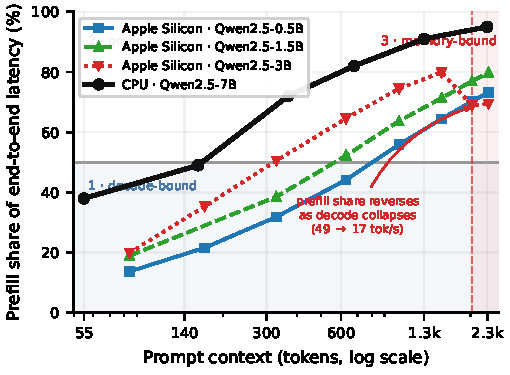
\includegraphics[width=\columnwidth]{fig_combined.pdf}
%   \caption{Prefill fraction against prompt length on both platforms.}
%   \label{fig:combined}
% \end{figure}

% =====================================================================
\section{Why They Differ}
\label{sec:why}
% =====================================================================

The mechanism is not subtle, which is part of why the inversion is worth stating plainly.

Prefill is a single pass over the whole context and is embarrassingly parallel across tokens; it is
compute-bound. Decode is sequential---each token depends on the last---and is bound by memory bandwidth, since
every step streams the weights and the growing KV cache~\cite{kwon2023pagedattention,agrawal2024sarathi}.

A CPU has little parallelism to bring to prefill, so prefill cost scales with context and comes to dominate
everything else. Apple Silicon's GPU parallelises prefill well, so prefill is comparatively cheap---up to
12$\times$ cheaper per token---which exposes decode's sequential cost instead. The datacentre disaggregation
literature separates these two phases precisely because they stress different
resources~\cite{patel2024splitwise,zhong2024distserve}; on-device, they stress \emph{different platforms}
differently, and there is nowhere to disaggregate to.

Unified memory then adds a second-order effect with a first-order consequence. On Platform~B, weights and KV
cache share one pool. Once their combined footprint approaches capacity, decode throughput does not taper---it
falls off a cliff, 49 to 13\,tok/s. Work on offloading weights from flash addresses a related
constraint~\cite{alizadeh2024llmflash}, but the behaviour we observe is a hard discontinuity in a device a user
is holding, not a throughput curve to be tuned.

This is why we describe the platforms as two \emph{regimes} rather than two points on one curve. In regime~A the
scarce resource is compute and the lever is context length. In regime~B the scarce resource is memory and the
lever is KV growth. An optimisation that helps in one is neutral or harmful in the other.

% =====================================================================
\section{What This Means for Mobile Systems}
\label{sec:implications}
% =====================================================================

\paragraph{1. Single-number benchmarks conceal the inversion.}
Reporting ``tokens per second'' collapses two phases with opposite scaling behaviour into one figure, and does
not say which phase produced it. A device reporting 12\,tok/s in regime~A and one reporting 12\,tok/s in
regime~B will behave completely differently as a user's context grows. We would argue on-device benchmarks
should report prefill and decode separately as a minimum, and prefill \emph{fraction} against context length by
preference. This is a cheap change to make and it is the one that would have prevented the intuition we started
with from propagating.

\paragraph{2. Placement and offload decisions inherit the wrong prior.}
Routing and cascade systems decide what runs where, and typically cost a request by expected output
length~\cite{chen2023frugalgpt,ong2024routellm,schuster2022calm}. On a CPU-class edge device that estimate is
close to irrelevant: the cost is in the input. A scheduler carrying a decode-bound prior will systematically
under-cost long-context requests on exactly the devices least able to absorb them.

\paragraph{3. The memory wall is a design constraint, not a tuning parameter.}
Because decode collapses rather than degrades, on-device capability is discontinuous. An application that
behaves well at 1{,}800 tokens of context may be unusable at 2{,}200 on the same hardware. That is an
application-architecture fact---it dictates how much history a mobile assistant can carry---and it cannot be
recovered by a runtime flag.

\paragraph{4. Context budgeting is a first-class lever.}
If latency is governed by what the model reads, then what it reads is the thing to control. We demonstrated this
on Platform~A: gating the costliest optional stage of an agent pipeline---a second ``review/verify'' model
pass---cut end-to-end latency \textbf{2.4$\times$} with no measurable quality loss under an order-swapped LLM
judge~\cite{zheng2023judging}. The lever is not a micro-optimisation; on that platform it is the largest single
one available, and it is invisible to anyone optimising decode.

\paragraph{5. Deployment advice should name its platform.}
Guidance of the form ``quantize down for speed'' is not wrong so much as unqualified. On Platform~A the 8-bit
build was fastest to prefill; on Platform~B the reason to quantize is to stay under the memory wall. The same
action is taken for opposite reasons, and stating which reason applies is the difference between advice that
transfers and advice that misleads.

% =====================================================================
\section{Open Questions}
\label{sec:open}
% =====================================================================

We would rather end with the questions we cannot answer than with a summary.

\paragraph{Where do NPUs sit?} Neither platform here includes a dedicated neural accelerator. An NPU may
constitute a third regime, or may land between the two---and if the number of regimes keeps growing, the case
for measurement over intuition strengthens rather than weakens.

\paragraph{Does the inversion survive architectural change?} Mixture-of-experts changes what is resident in
memory during decode; speculative decoding changes the sequential dependency that makes decode
slow~\cite{leviathan2023speculative}. Both act directly on the mechanism we describe. Whether they narrow the
gap between regimes or widen it is an empirical question we have not answered.

\paragraph{Can a runtime detect its own regime and adapt?} This is the question we find most interesting. The
signals are cheap to obtain---prefill fraction, decode throughput, memory headroom---and the corresponding
actions are known: budget context when compute-bound, cap KV growth when memory-bound. A runtime that measured
its own regime at startup and adapted its policy accordingly would need no platform-specific tuning by the
developer. We do not know whether such a controller is stable in practice, and we think it is worth finding out.

\paragraph{Limitations.} Both studies are single-machine per platform, with a second CPU vendor as the only
cross-device check. We measure three model families at one primary quantization level each. Absolute numbers
should be read as characteristic of these devices; the \emph{inversion} is the claim we defend, and it survives
across models and across two CPU vendors.

% =====================================================================
\section{Conclusion}
% =====================================================================

On-device LLM latency has no platform-independent characterisation. On CPU-class hardware, prefill dominates and
the binding constraint is compute. On memory-constrained Apple Silicon, the balance inverts and the binding
constraint is memory, with a hard discontinuity once the KV cache stops fitting. Any system that schedules,
places, or budgets on-device inference---and any benchmark that reports its speed---should measure the hardware
rather than inherit an intuition from a datacentre it will never run in.

% =====================================================================
\section*{Reproducibility}
\label{sec:repro}
% =====================================================================

Both harnesses, all raw per-run data, and the analysis scripts are public.

\begin{itemize}\itemsep2pt
  \item CPU study\\
        \texttt{\small github.com/bapista/cpu-llm-latency}\\
        DOI 10.5281/zenodo.21765705
  \item Apple Silicon study\\
        \texttt{\small github.com/bapista/mlx-llm-latency}\\
        DOI 10.5281/zenodo.21786211
\end{itemize}

Every number in this paper traces to a line in a released results file. Earlier versions of both studies are
available as preprints at the DOIs above.

\bibliographystyle{ACM-Reference-Format}
\bibliography{references}

\end{document}
